\section{Teaching philosophy and aims of the course}


\section{How mathematical models make sense of complex processes}

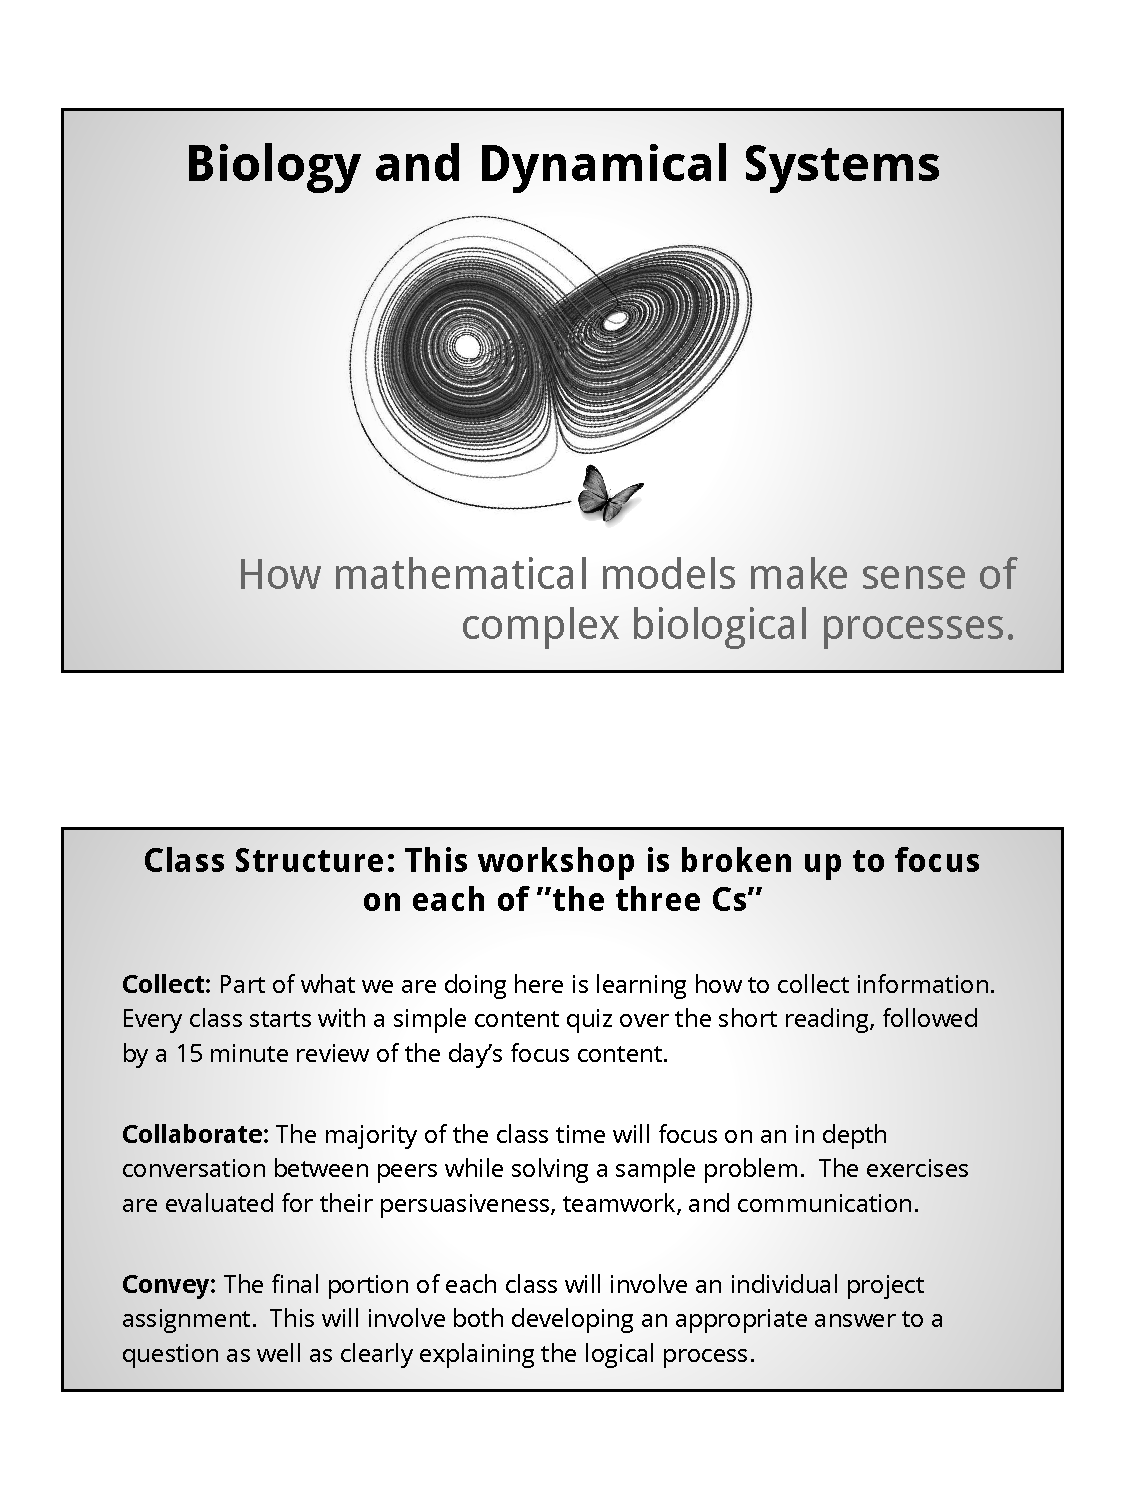
\includepdf[pages={1-}]{workshop/wk1_intro_and_cartoons.pdf}


\section{Modeling biological systems with differential equations}
\paragraph{``Modelling biological systems} is a significant task of systems biology and mathematical biology. It involves the use of computer simulations of biological systems, including cellular subsystems (such as the networks of metabolites and enzymes which comprise metabolism, signal transduction pathways and gene regulatory networks), to both analyze and visualize the complex connections of these cellular processes.'' --Wikipedia

\paragraph{Many types of models} Biological models can work in many different ways:  In general, models are made to focus on systems at a certain scale.  We can choose from a wide variety of model types. Some work by modeling continuous values, such as concentration of a protein.  Others work by modeling the discrete state of a system, such as a neuron being either on or off.  Some models are deterministic, meaning that there is no randomness, while others add stochastic noise.

\paragraph{Focusing on Differential equations} In our class we?re going to focus on probably the simplest and most widely used kind of mathematical model, differential equations.  Differential equations are a continuous, deterministic model, they model real values with rules that describe exactly how those values change.  Differential equations are very similar to the equations we learned about in our high school and college calculus courses.

\paragraph{What is a differential equation good for?} A differential equation is a simple formula that describes how a system will change in time based on the state of the system right now. You can think of it like a very formal protocol for how concentrations of substances will change over time.  For example, a differential equation 

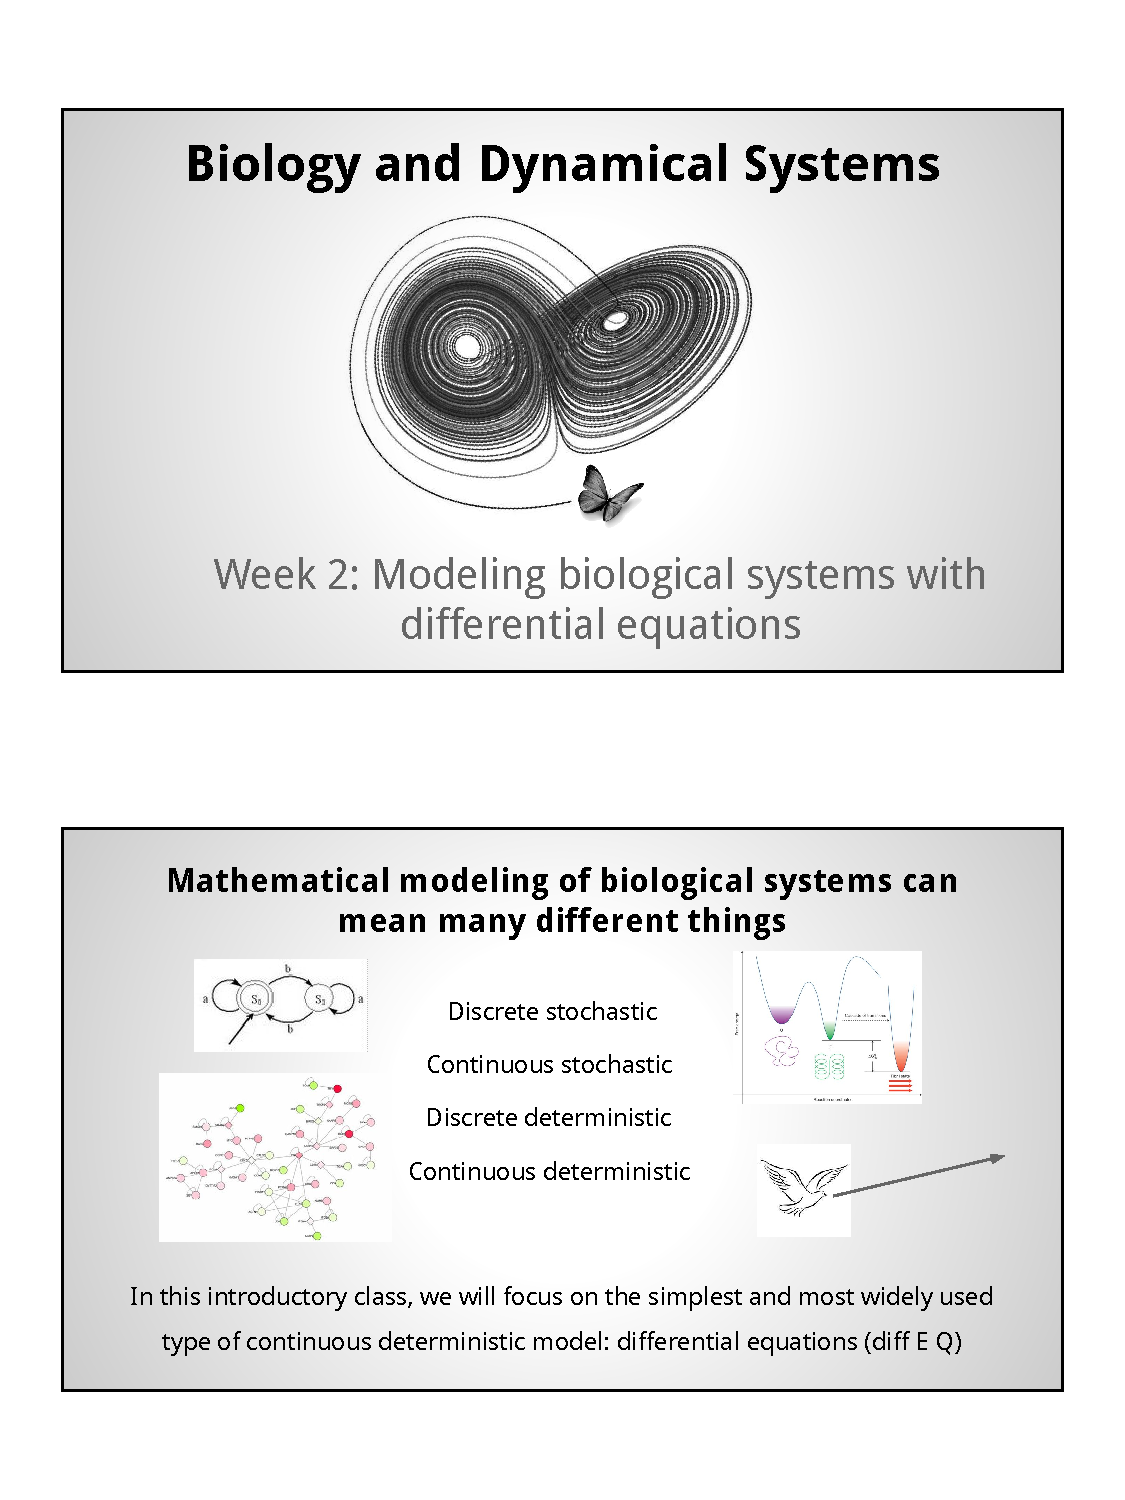
\includepdf[pages={1-}]{workshop/wk2_diff_eq.pdf}



\section{Visualizing equations with graphs}
\paragraph{Why is it called differential?} One could argue that differential equations could actually be called derivative equations.  That?s because the equation itself is really just a way of explicitly writing out the derivative of a variable.  For those that don?t remember a derivative is just ?a way to represent rate of change, that is - the amount by which a function is changing at one given point...it is the slope of the tangent line at a point on a graph.?

\paragraph{Equilibrium?} Another important concept in diffeq is that of equilibrium.  The meaning of equilibrium is simple once you have a rate equation to look at.  When the net rates of change of all variable are equal to 0, then nothing can change anymore.  The rates of production and destruction are balanced, and the concentrations of everything will remain constant forever.  Not all systems reach equilibrium, but most do, and finding equilibria is the first step to understanding how many systems work.  We will use equilibrium and steady state more or less interchangeably though there are subtle, pedantic differences.

\paragraph{Initial conditions and transient behaviors} Even though most systems reach equilibrium after a long time, the system?s initial conditions set the early ?transient? behavior. The initial condition, or seed value, is simply the state of the system where we choose to start.  The transient behavior is the way in which the system changes from the initial conditions to the steady state.

\paragraph{What are nullclines?} If our rate equation has two variables that can change in it (i.e. not constants), then there is no longer a single value at which the rate equation will equal 0.  Instead there will be a set of values that make the rate 0.  This set of values defines a line, and this line is called a nullcline. 
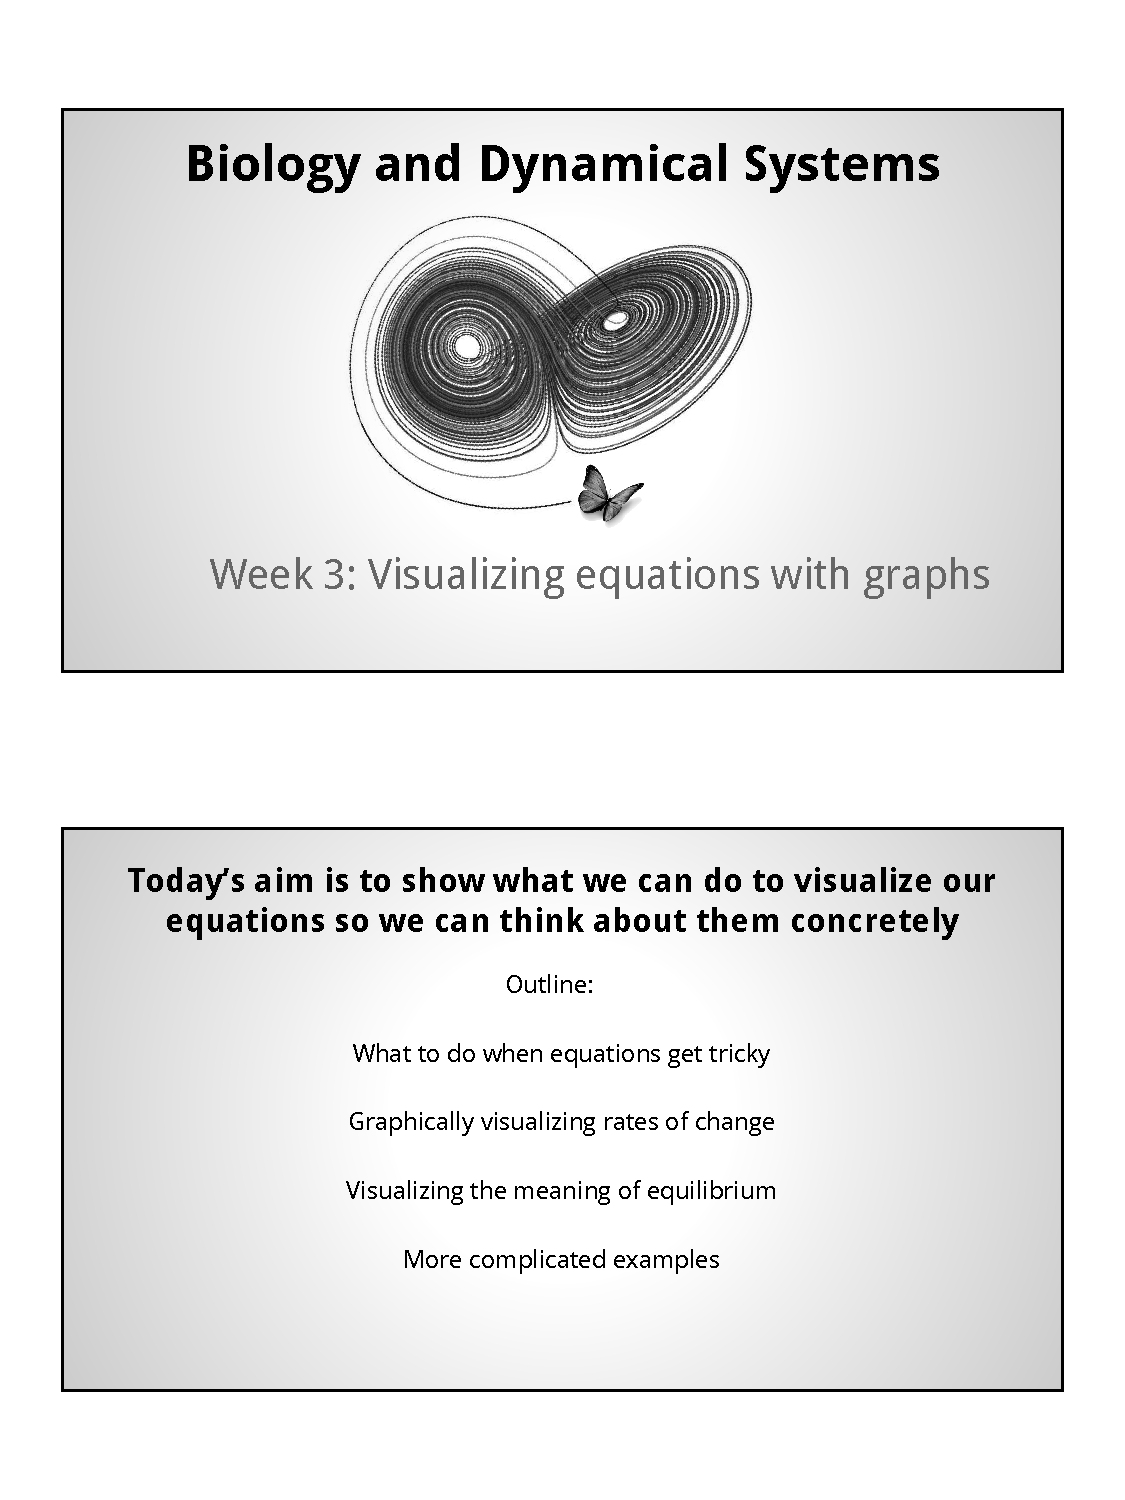
\includepdf[pages={1-}]{workshop/wk3_diag.pdf}



\section{Simplifying models and starting simulations}
\paragraph{Why simplify before simulating?} There are a number of reasons to simplify your equations before you ever start a simulation.  Here are my top three.  
1) You won?t be able to remember or adequately describe all the parameters that went into a given simulation when somebody asks you.  If you have 20 parameters in a simulation there will always be a huge risk that you screwed one of them up and you will never be able to notice.  
2) If you want to understand how your model works under many different conditions, then every time you add a parameter you have to do exponentially more work.  In other words, when you are systematically checking how 3 parameters work together you may have to do $100^3$ different simulations and analyze your results.  If you add one more parameter you will have to do $100^4$ simulation or 100 times more work.  
3) Nobody wants to look at a disorganized giant equation.  If you have a complicated equation most people will decide it isn?t worth their time to pay attention to the modeling so none of your modeling work will count for anything anyway.

\paragraph{The parts of a differential equation model} A differential equation model can be broken down into 3 parts: variables, parameters, and the form of the equation.  Variables are the values (like concentration) that are changing in time.  This is the physically ?real? stuff like the number of proteins or the size of your cell.  Parameters are things like rate constants and diffusion coefficients.  These are descriptive numbers that set the magnitudes of rates of change.  Finally, the form of the equation determines how the variables and parameters fit together.  This is the level at which we can see how each variable affects the other qualitatively, but it takes parameters to know by how much.

\paragraph{How do simulations work?} The applied math behind solving differential equations with computers is rich and we certainly won?t understand everything that has been done over the past 70 years to solve these problems.  However we can get some intuition by looking at the simplest way of solving, called the Euler method.  In this method you ?step? through time and change the value of your variables by a small amount using the rules defined in your differential equation (See wikipedia page for more info).  If you ever try this, you will get bored very fast because it is really annoying.  But when computers do this, they can take very small steps and therefore ?solve? the system with arbitrary accuracy.  There have been a bunch of modifications of this technique that significantly improve the accuracy vs timestep tradeoff.


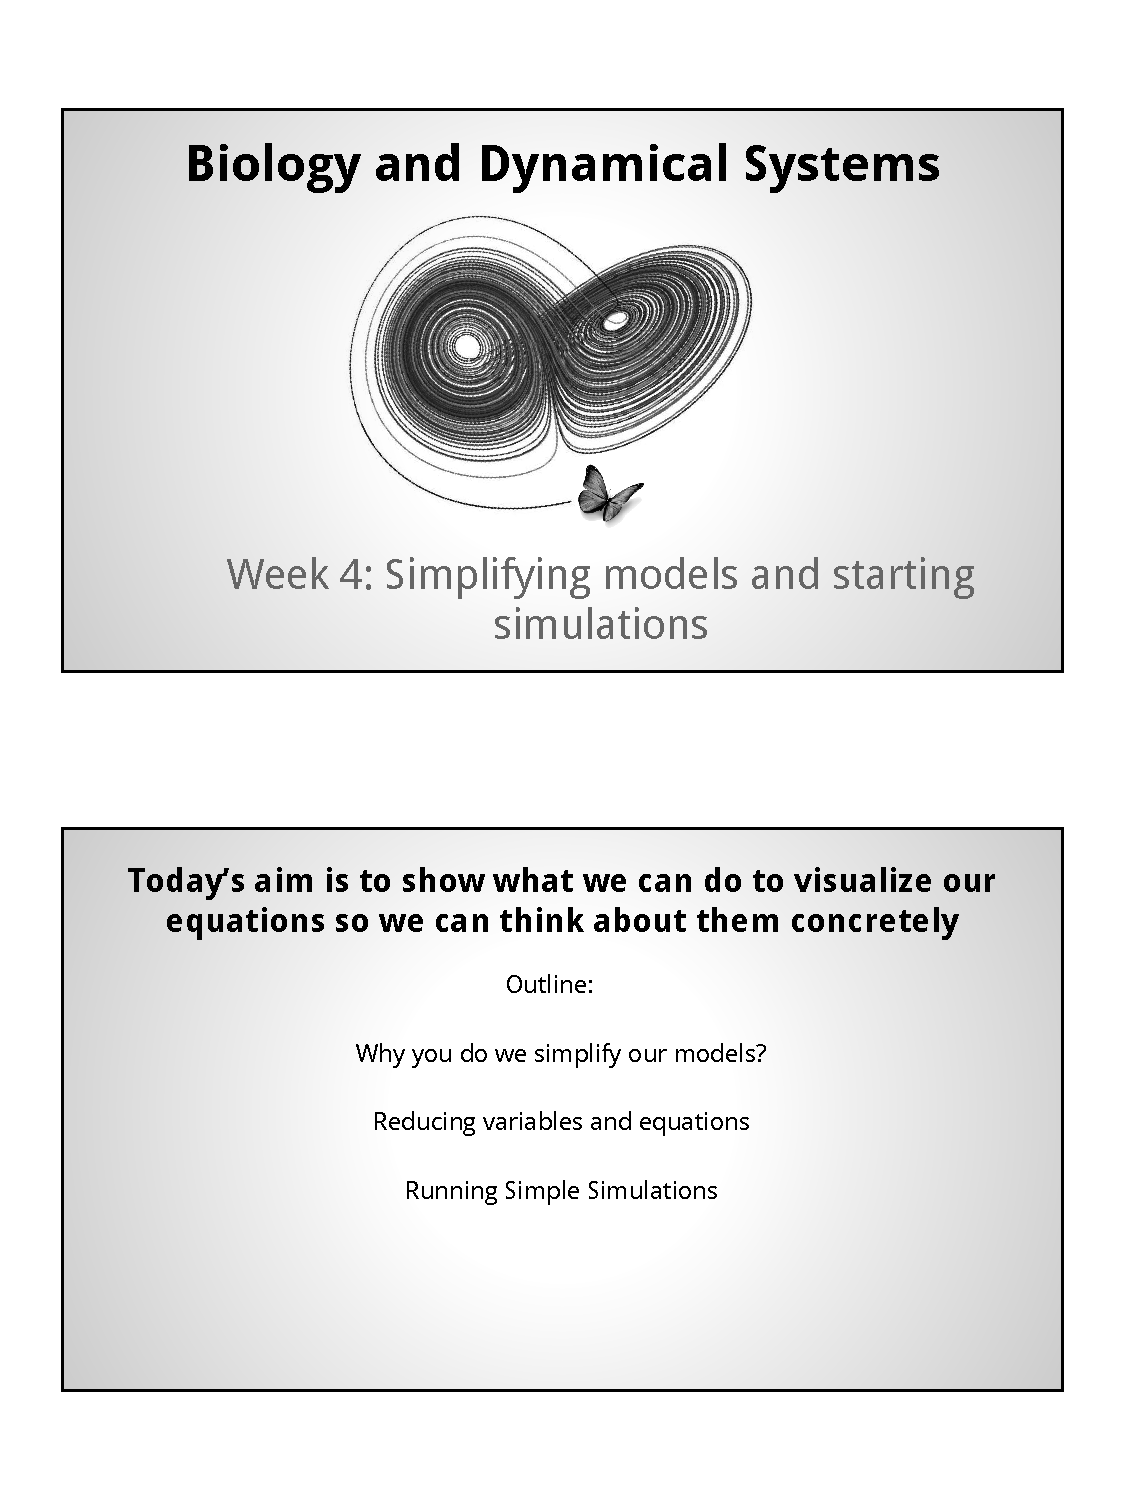
\includepdf[pages={1-}]{workshop/wk4_simple.pdf}



\section{Analyzing equations and understanding simulation output}

\paragraph{(from wikipedia) Nondimensionalization} is the partial or full removal of units from an equation involving physical quantities by a suitable substitution of variables. This technique can simplify and parameterize problems where measured units are involved. It is closely related to dimensional analysis. In some physical systems, the term scaling is used interchangeably with nondimensionalization, in order to suggest that certain quantities are better measured relative to some appropriate unit. These units refer to quantities intrinsic to the system, rather than units such as SI units. Nondimensionalization is not the same as converting extensive quantities in an equation to intensive quantities, since the latter procedure results in variables that still carry units.

\paragraph{Running simulations}: The following two snippets of code is all you need to solve differential equations in MATLAB.


\begin{verbatim}
function dc = myode(t,p,a,b)
    p1 = p(1);
    p2 = p(2);
    dp1 = 1 - a*p2 - p1;
    dp2 =p1 - b*p2;
    dp = [dp1;dp2];
end
\end{verbatim}

\begin{verbatim}
t = 0:0.1:10;      #timepoints for solution (1 to 10 increment of 0.1)
p0 = [1,0];         #initial conditions for the concentration of p1 and p2
a=1; b=1;          #optional constants a and b which will change behavior
[t, pt] = ode45(@myode,t,p0,[],a,b);        #this runs the simulaton 
plot(t,p(:,1)); hold on; plot(t,p(:,2));           #this plots the output
\end{verbatim}

So now you can put whatever you want into the equation and change your parameters and run many simulations.  

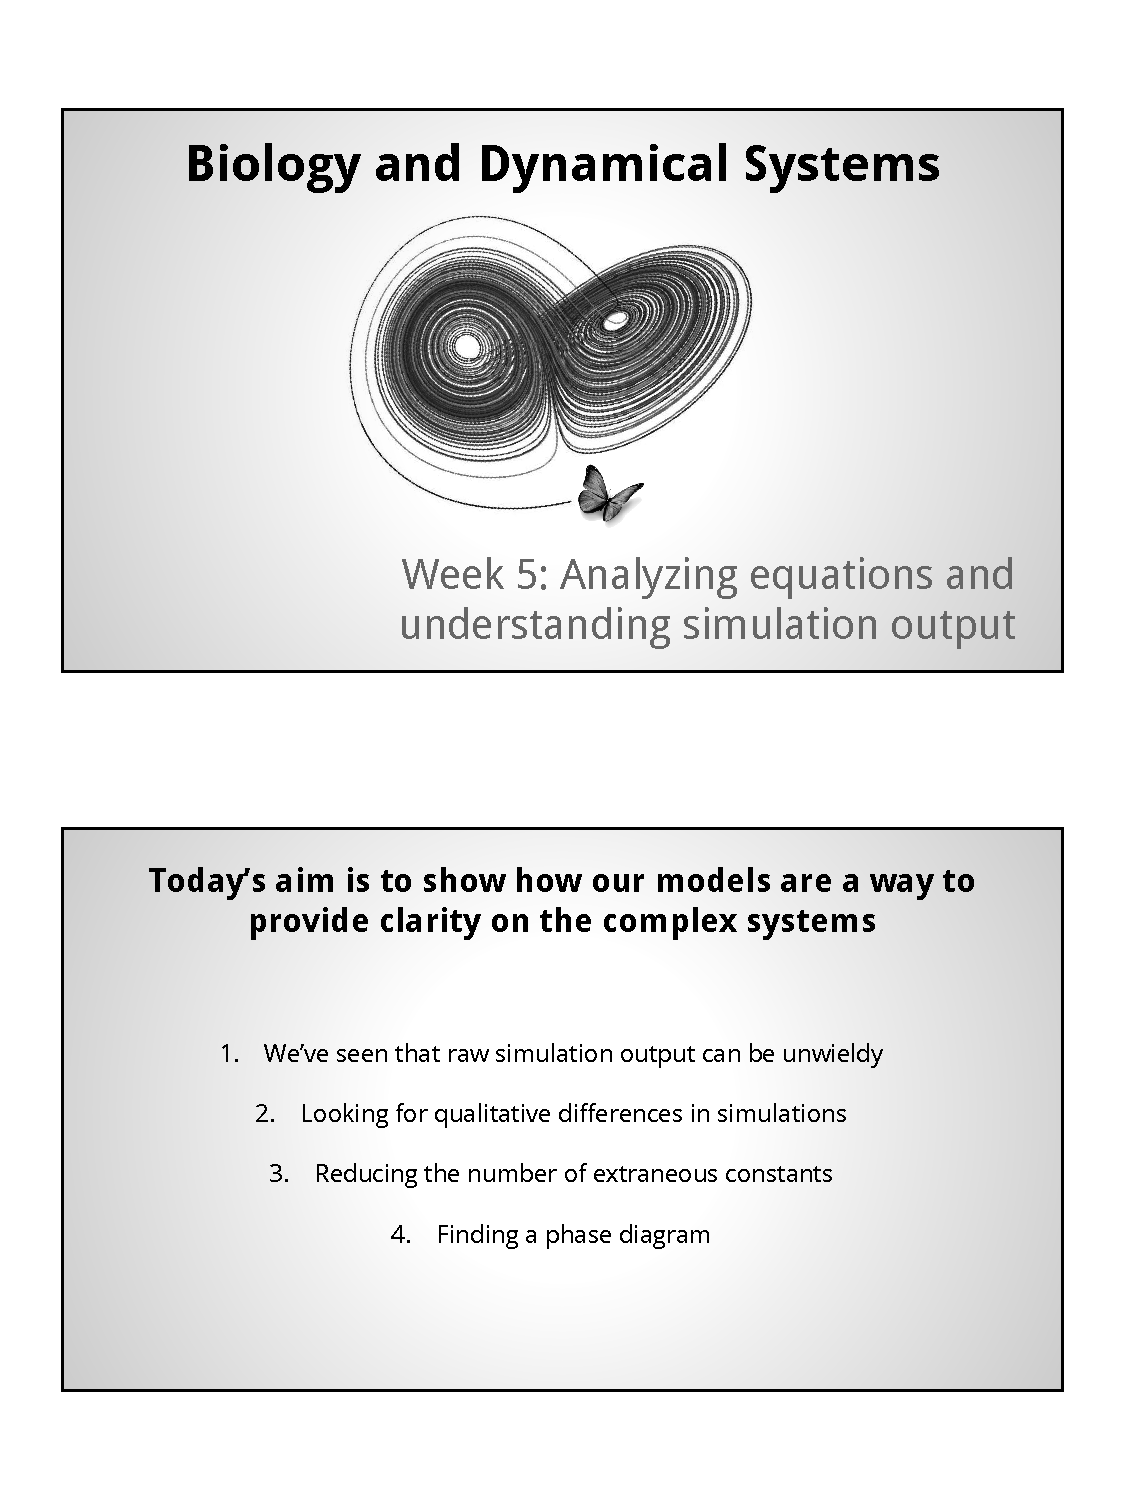
\includepdf[pages={1-}]{workshop/wk5_analysis.pdf}



\section{Explaining ever more complex systems}

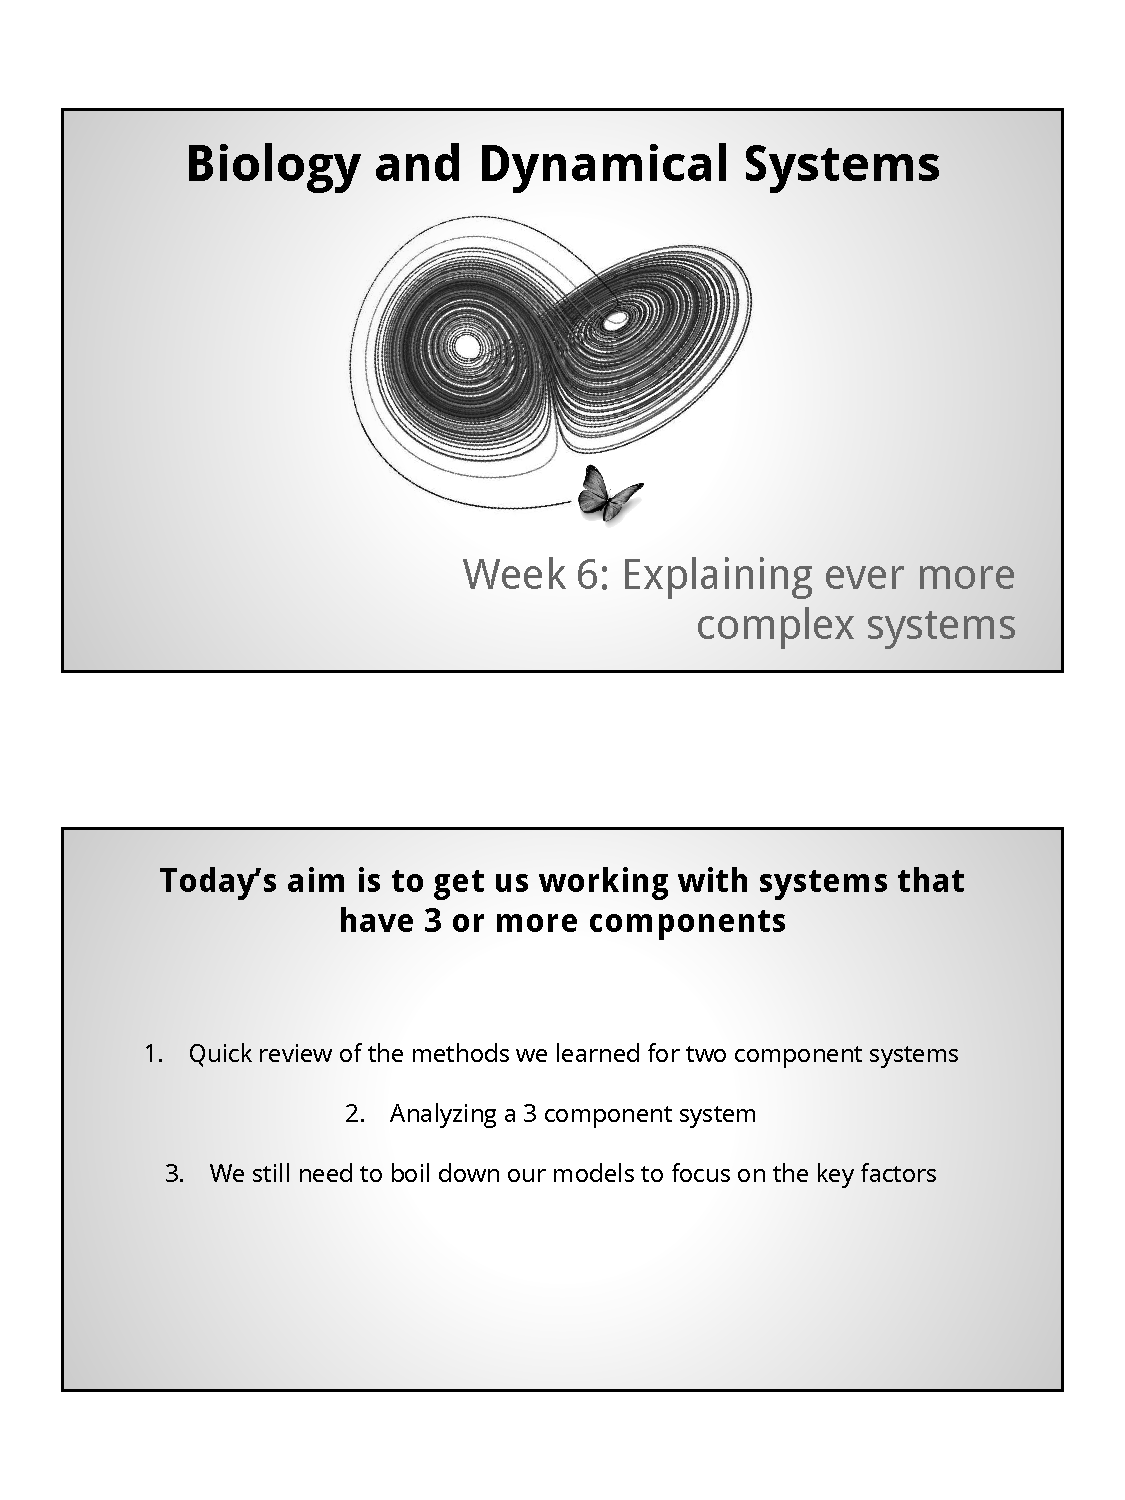
\includepdf[pages={1-}]{workshop/wk6_display.pdf}


\section{Thoughts and Student Responses}

\section{Quizzes and Project ideas}
\paragraph{W2}
Q1: Which is not a situation that is amenable to mathematical modeling?
A metabolism, signal transduction pathways, gene regulatory networks, protein purification

Q2: Which is a category of biological mathematical model?
A soft, prescient, discrete, topological

Q3: Which type of model is a differential equation?
A continuous deterministic, discrete stochastic, continuous stochastic, discrete deterministic

Q4: What does a differential equation most closely resemble?
A a protocol, a patent, a dissertation, a legume


\paragraph{W3}
Q1: Which is the closest synonym for derivative in the context of diffeq?
A Unoriginal, by-product, change, sum

Q2: Which is least similar to equilibrium?
A balanced rates, constant concentrations, discrete probabilities, steady states

Q3: Which conditions set the transient behavior?
A initial, parametric, hyperbolic, final

Q4: Nullclines are...
A topographical, unimportant, lines, esoteric

\paragraph{W4}
Q1: Number of simulations to run varies --- with the number of free parameters.
A quadratically, logarithmically, exponentially, combinatorially

Q2: Which is not a part of a differential equation model?
A definitions, variables, parameters, the form of the equation

Q3:The Euler method gives exact solutions.
A True, False, neither, depends who you ask

Q4: Who likes looking at a disorganized mess of an equation?
A Your PI, your colleagues, your reviewer, nobody

\paragraph{W5}
Q1: Once nondimensionalization is complete?
A All variables have units of time, there are no more parameters left, equations are simpler to analyze, your solutions will fall on a line

Q2: In MATLAB --- is the function for solving differential equations
A ode23tb, ode113, ode45, ode15i

Q3: Which isn?t necessary to solve a differential equation
A An ode function, constants, initial conditions, timepoints for solution
